% vis-cycle.tex
% ref: http://texblog.net/latex-archive/uncategorized/pgf-tikz-commutative-diagram/

\documentclass[tikz]{standalone}
\usetikzlibrary{chains, arrows.meta, positioning, decorations.pathmorphing, decorations.pathreplacing}

\newcommand{\so}{\texttt{so}_{A}}
\newcommand{\lvo}{\texttt{lvo}_{A}}
\newcommand{\rvo}{\texttt{rvo}_{A}}

\makeatletter
\tikzset{join/.code=\tikzset{after node path={%
\ifx\tikzchainprevious\pgfutil@empty\else(\tikzchainprevious)%
edge[every join]#1(\tikzchaincurrent)\fi}}}
\makeatother

\tikzset{>=stealth,every on chain/.append style={join},
         every join/.style={->}}

\begin{document}
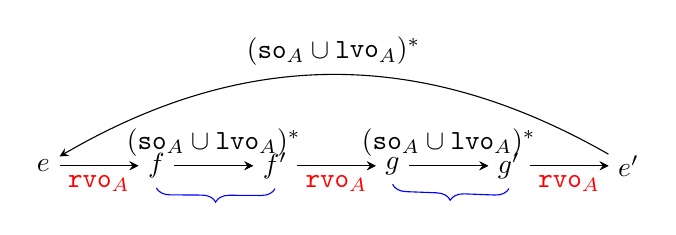
\begin{tikzpicture}[start chain] {
    \node (e) [on chain] {$e$};
    \node (f) [on chain, join = {node [below, red] {$\rvo$}}] {$f$};
    \node (f') [on chain, join = {node [above] {$(\so \cup \lvo)^{\ast}$}}] {$f'$};
    \node (g) [on chain, join = {node [below, red] {$\rvo$}}] {$g$};
    \node (g') [on chain, join = {node [above] {$(\so \cup \lvo)^{\ast}$}}] {$g'$}; 
    \node (e') [on chain, join = {node [below, red] {$\rvo$}}] {$e'$}; 

    % \node (h') [above left = 0.50cm and 0.50cm of e'] {$h'$};
    % \node (h) [above right = 0.50cm and 0.50cm of e] {$h$};
    % 
    % \draw [->] (e') to [above] node [sloped] {$\lvo$} (h');
    % \draw [->] (h') to [above] node [sloped] {$(\so \cup \lvo)^{\ast}$} (h);
    % \draw [->] (h) to [above] node [sloped] {$\lvo$} (e);

    \draw [->, bend right] (e') to node [above, sloped] {$(\so \cup \lvo)^{*}$} (e);

    \draw [blue, decorate, decoration = {brace, amplitude = 5pt, mirror}]
	(f.south) to node [below] {} (f'.south);
    \draw [blue, decorate, decoration = {brace, amplitude = 5pt, mirror}]
	(g.south) to node [below] {} (g'.south);
%     \draw [blue, decorate, decoration = {brace, amplitude = 5pt, raise = 45pt}]
% 	(e.north) to node [below] {} (e'.north);
  }
\end{tikzpicture}
\end{document}